\documentclass{article}
\usepackage{graphicx}
\graphicspath{ {./} }
\usepackage{color}

\usepackage{amsmath}
\usepackage{commath}
\usepackage{amssymb}
\usepackage{listings}
\usepackage{algorithm2e}
\usepackage{float}

\usepackage{hyperref}
\hypersetup{linktoc=all}

\usepackage{listings}
\usepackage{geometry}
\geometry{margin=1in}
\usepackage{color}
\definecolor{light-gray}{gray}{0.95}
\lstset{numbers=right,
                basicstyle=\tiny,
                numberstyle=\tiny,
                breaklines=true,
                backgroundcolor=\color{light-gray},
                numbersep=5pt,
                xleftmargin=.5in,
                xrightmargin=.5in}

\sloppy
\definecolor{lightgray}{gray}{0.5}
\setlength{\parindent}{0pt}

\begin{document}

\title{Lab 4: Detecting Image Editing}
\author{Brian Hosler \& Sarah Peachey }
\maketitle

\qquad words about intro jawn 

\newpage



\section{Detecting Image Contrast Enhancement}

\qquad words about stuff for part one 

\begin{verbatim}
ce1=imread('Assignment6Files/imageCE1.tif');
ce2=imread('Assignment6Files/imageCE2.tif');
ce3=imread('Assignment6Files/imageCE3.tif');
ce4=imread('Assignment6Files/imageCE4.tif');
ce5=imread('Assignment6Files/imageCE5.tif');

subplot(1,2,1)
imhist(ce1)%ENHANCED
subplot(1,2,2)
imhist(ce2)
figure
subplot(1,2,1)
imhist(ce3)%ENHANCED
subplot(1,2,2)
imhist(ce4)

ui1=imread('Assignment6Files/unaltIm1.tif');
ui2=imread('Assignment6Files/unaltIm2.tif');
ui3=imread('Assignment6Files/unaltIm3.tif');

figure
subplot(3,1,1)
imhist(Gcorrection(ui1,.7))
subplot(3,1,2)
imhist(ui1)
subplot(3,1,3)
imhist(Gcorrection(ui1,1.3))

figure
subplot(3,1,1)
imhist(Gcorrection(ui2,.7))
subplot(3,1,2)
imhist(ui2)
subplot(3,1,3)
imhist(Gcorrection(ui2,1.3))

figure
subplot(3,1,1)
imhist(Gcorrection(ui3,.7))
subplot(3,1,2)
imhist(ui3)
subplot(3,1,3)
imhist(Gcorrection(ui3,1.3))

figure
imhist(ce5)

type('Gcorrection.m')
\end{verbatim}

\color{lightgray} \begin{verbatim}
function [ img_out ] = Gcorrection(img_in, gama)
%Does gamma correction using the equation:
%   new=2558(old/255)^gamma
    img_out=uint8(255*(double(img_in)/255).^gama);
end

\end{verbatim} \color{black}
    
words about resutlts from part 1 


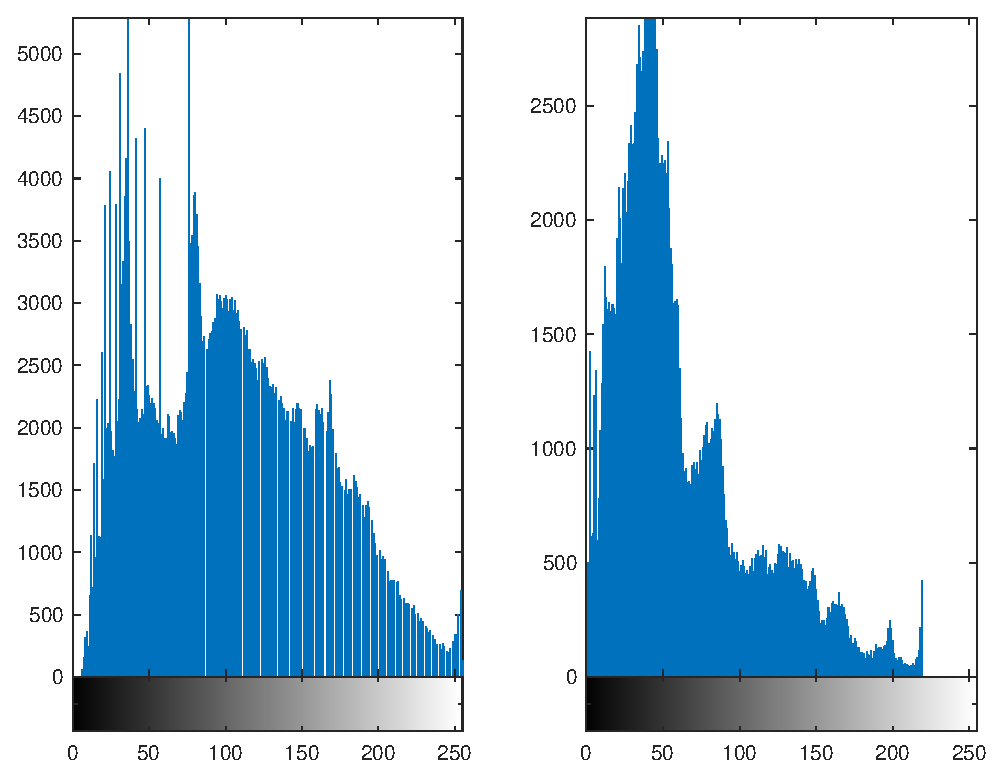
\includegraphics [width=4in]{lab6_01.eps}

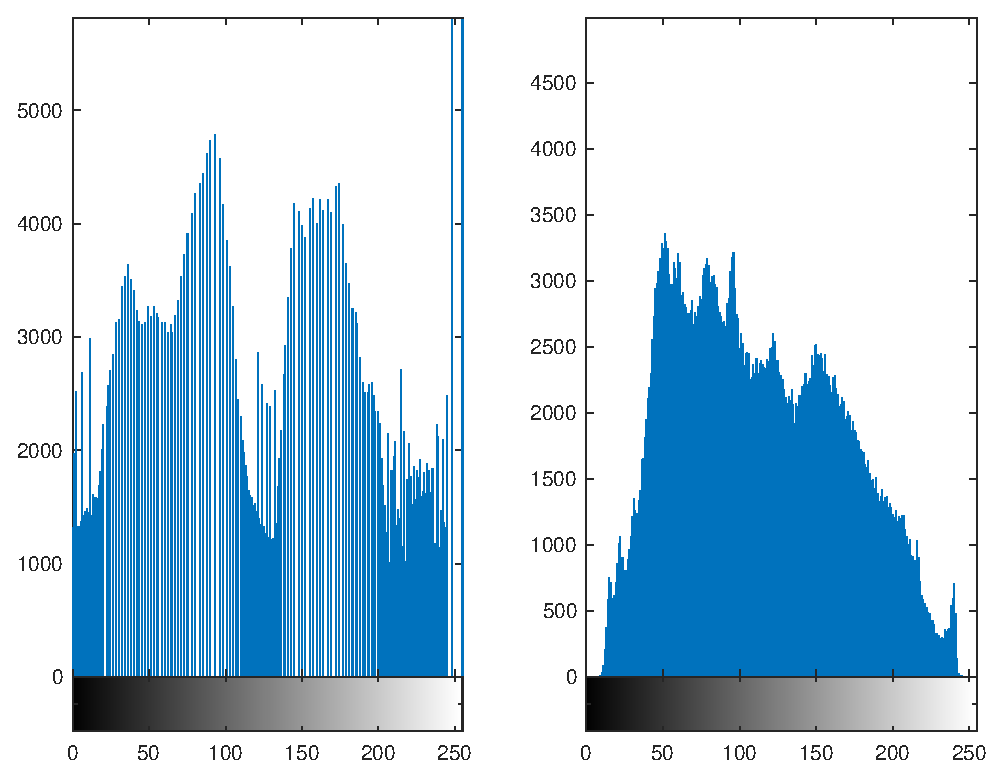
\includegraphics [width=4in]{lab6_02.eps}

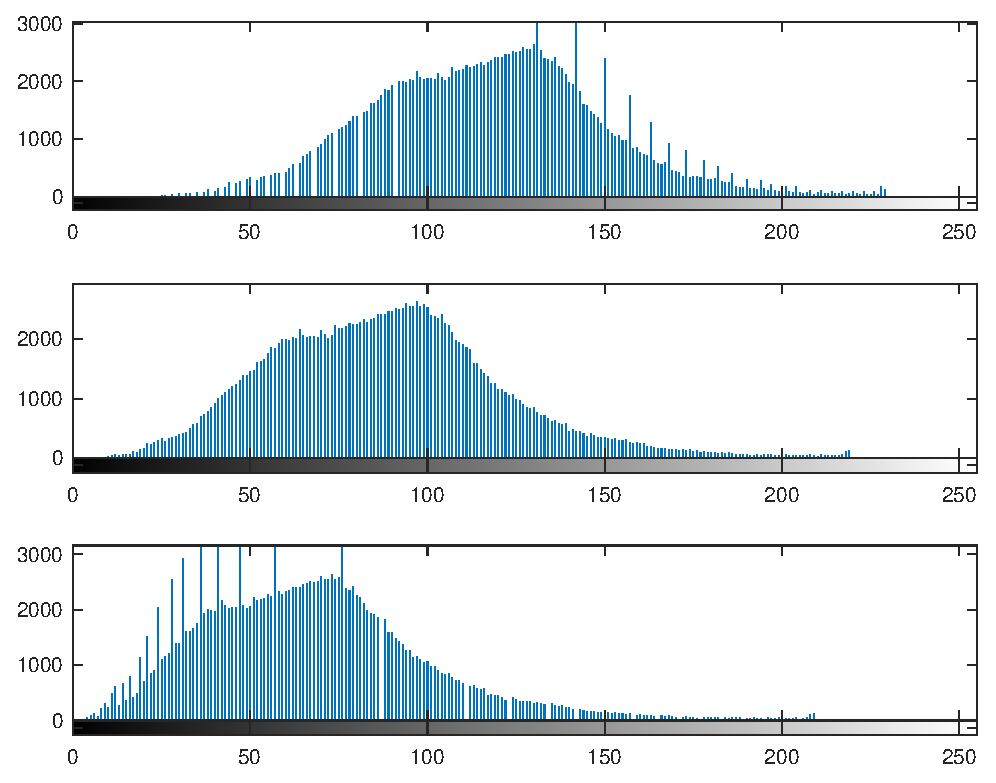
\includegraphics [width=4in]{lab6_03.eps}

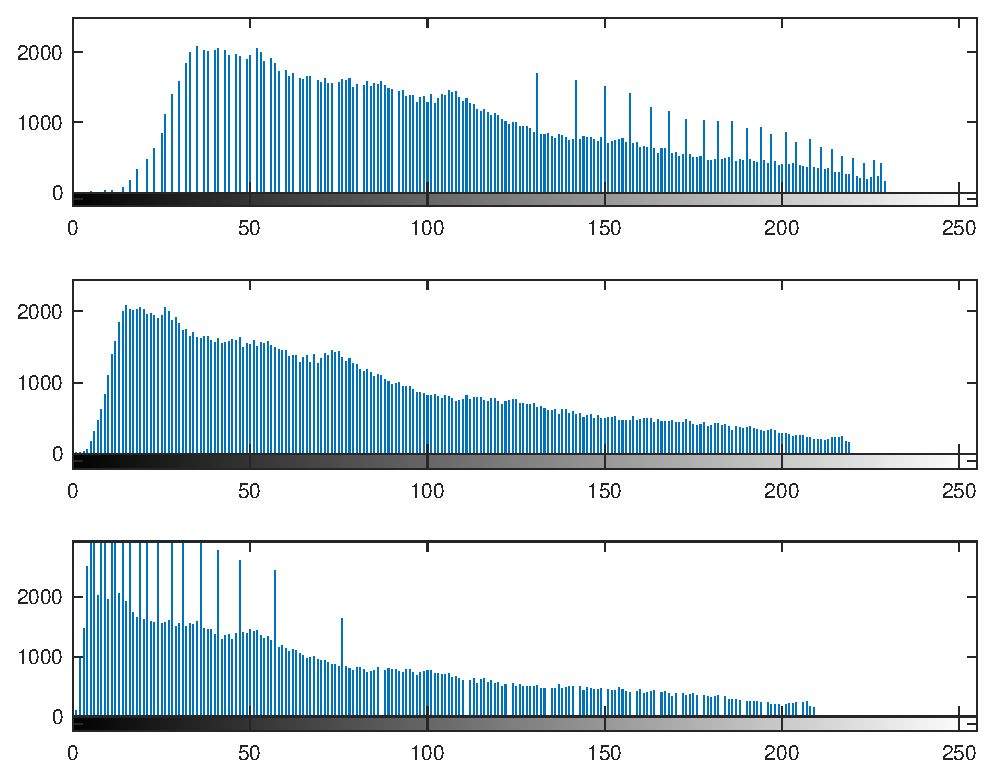
\includegraphics [width=4in]{lab6_04.eps}

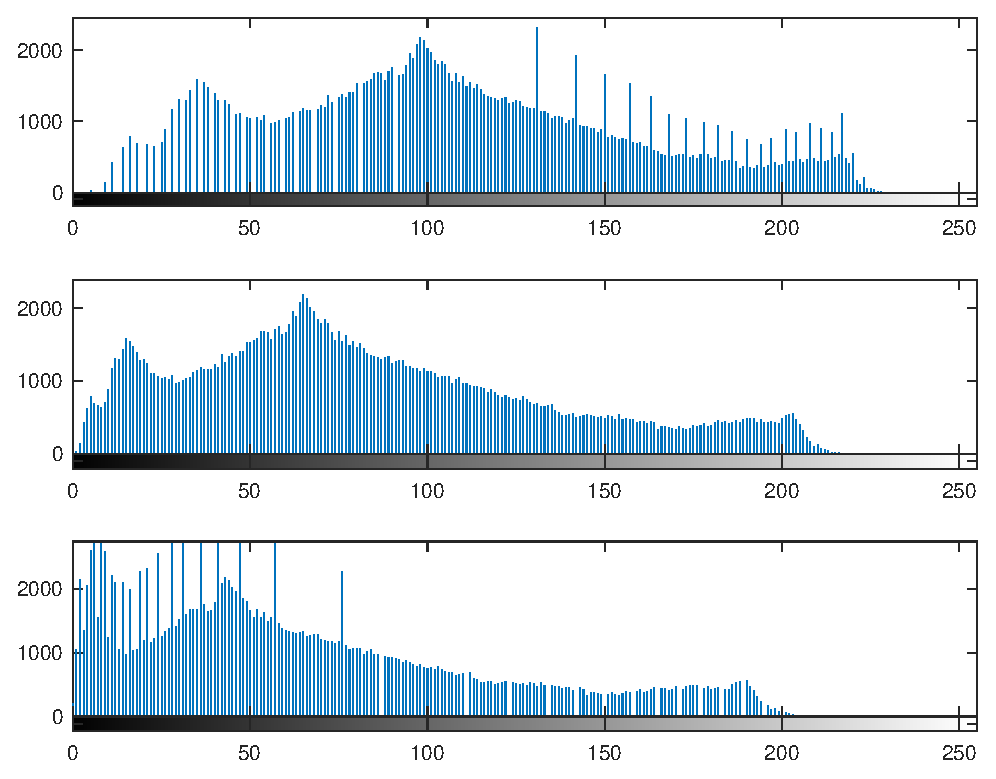
\includegraphics [width=4in]{lab6_05.eps}

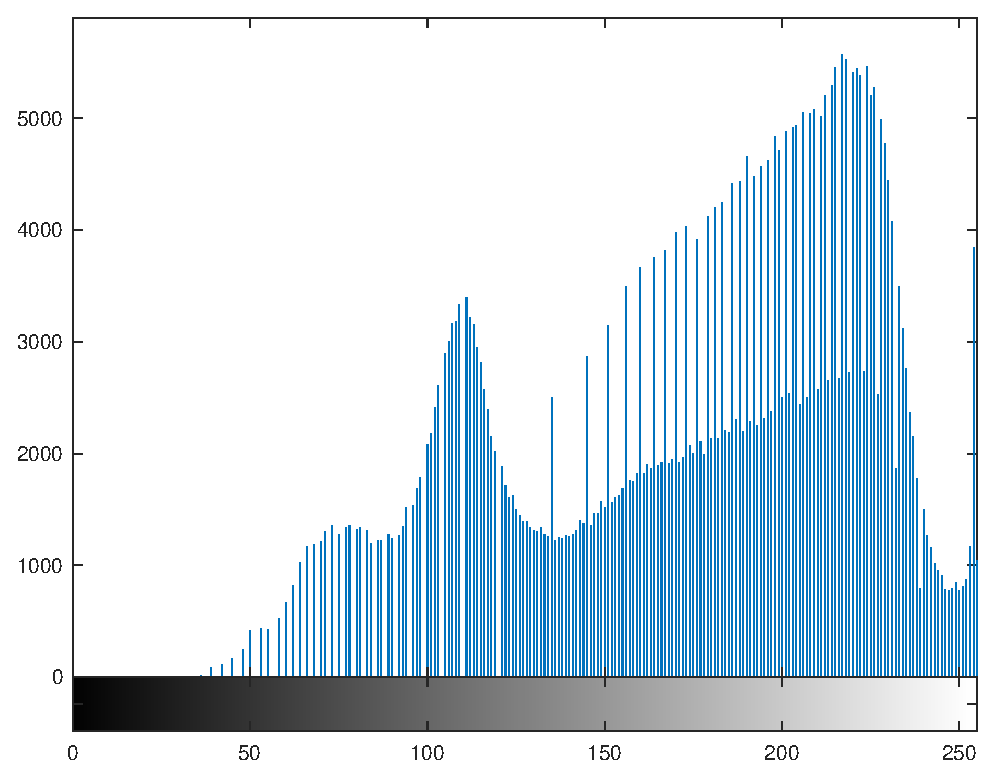
\includegraphics [width=4in]{lab6_06.eps}


\section{Detecting Image Resampling and Resizing}

\qquad One of the most common image resampling operations is resizing. Image
resampling fingerprints can be detected with the Popescu and Faird method
but is computationally complex. The algorithm derived by Kirchner is an
approximation of the same results but far less computationally intense. 
Kirchner's algorithm uses a fixed linear filter to approximate relationships
between pixel values. The variance resulting from the predicted pixel error
will be periodic. As seen in the below function Kirchner's algorithm, the
image is first filtered with the linear prediction filter, then the error is
calculated, and the p-map is then approximated with the below equation. 
 
\begin{align} 
	p(x,y)=\lambda exp^{\frac{-e(x,y)^\tau}{\sigma}}
\end{align}



\color{lightgray} \begin{verbatim}
function [ pmap_approx ] = kirchners( im )
%KIRCHNERS  approximates the pmap 
%   Detailed explanation goes here
I=double(im); 
% 1)
alpha=[-0.25 0.5 -0.25; 0.5 0 0.5;-0.25 0.5 -.25]; 
I_hat=filter2(alpha, I); 
% 2)
pred_error=I-I_hat; 
% 3)
lambda=1; 
tau=2; 
sigma=1; 
pmap_approx=lambda*exp((-pred_error.^tau)./sigma); 
end
\end{verbatim} 

\begin{verbatim}
im1=imread('Assignment6Files/resamp1.tif');
im2=imread('Assignment6Files/resamp2.tif');
im3=imread('Assignment6Files/resamp3.tif');
im4=imread('Assignment6Files/resamp4.tif');
p1= kirchners( im1 );
p2= kirchners( im2 );
p3= kirchners( im3 );
p4= kirchners( im4 );

figure
subplot(2,2,1)
imagesc(p1)
colormap(cool)
subplot(2,2,2)
imagesc(p2)
subplot(2,2,3)
imagesc(p3)
subplot(2,2,4)
imagesc(p4)

figure
subplot(2,2,1)
showFreqPmap(p1)
subplot(2,2,2)
showFreqPmap(p2)
subplot(2,2,3)
showFreqPmap(p3)
subplot(2,2,4)
showFreqPmap(p4)
type('kirchners.m')
\end{verbatim}\color{black}
    

Below shows the p-map for the several images, the top-left and bottom-right
images appear to have a periodic grid, so they are clearly resized. So just
based off the p-maps resampIm2.tif and resampIm3.tif appear to be resized
but the other two do not. But then the frequency of the p-map is calculated
which showed that the not only 2 and 3 but also resampIm4.tif was resampled
in at least one direction. 


\includegraphics [width=4in]{lab6_07.eps}

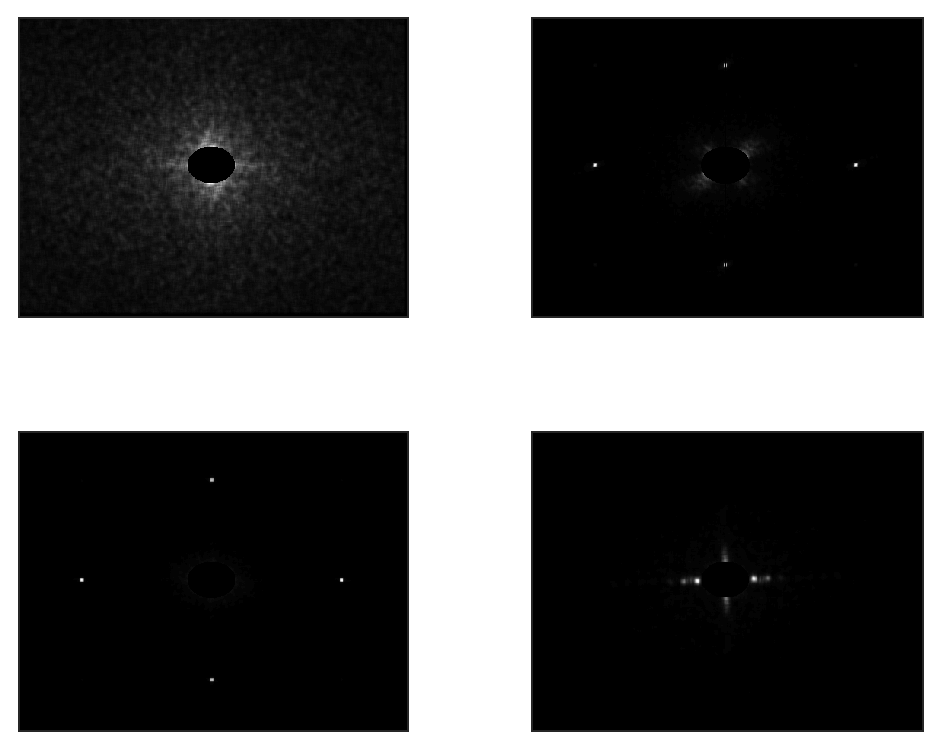
\includegraphics [width=4in]{lab6_08.eps}



\end{document}
    
